\section{Shellcode}
\subsection{Definition}
Um das folgende Beispiel besser zu verstehen, sollte zunächst erklärt werden, was genau Shellcode ist und wofür er benutzt wird.
Shellcode ist definiert als eine Folge von Anweisungen, die über einen Exploit in einen Prozess injiziert und
dann durch diesen ausgeführt werden. Er wird verwendet, um die Funktionalität eines Prozesses zu verändern und
Befehle auf einem Zielsystem auszuführen. In der Computersicherheit bedeutet Shellcoding im ursprünglichen Sinne,
das Schreiben von Code, der bei der Ausführung eine Remote-Shell öffnet. Die Bedeutung von Shellcode hat sich jedoch weiterentwickelt und
beschreibt mittlerweile jeden Byte-Code, der in einen Exploit eingefügt wird, um eine gewünschte Aufgabe zu erfüllen.

Zwar ist es theoretisch möglich Shellcode in höheren Programmiersprachen zu schreiben, in der Praxis ist die effizienteste und
fast ausschließlich verwendete Sprache jedoch Assembly. Dies ermöglichte, so maschinennah wie möglich zu arbeiten,
um mehr Kontrolle über Abläufe zu haben und Speicherplatz zu sparen. Der verfügbare Speicher für Shellcode ist meist limitiert.
Da Shellcode in Assembly geschrieben wird, ist es wichtig zu beachten, auf welcher Hardware und auf welchem Betriebssystem dieser laufen soll.
Es bestehen klare Unterschiede zwischen Linux- und Windows Shellcode: Unter Linux hat man überwiegend direkten Zugriff auf Interface und Kernel,
was unter Windows in der Regel nicht möglich ist. Im Folgenden wird ein Shellcode-Beispiel für 64Bit Unix Systeme betrachtet. \cite{tutorial1}

\subsection{Beispiel}

Das folgende Shellcode Beispiel ermöglicht es eine Shell auf dem ausführenden System zu öffnen und diese über eine Netzwerkverbindung fernzusteuern. 
Der Code umfasst dabei lediglich 29 Bytes, da dieser meist so effizient und klein wie möglich sein sollte. 
Am besten lässt sich die Erklärung von unten, also mit dem Syscall, beginnen. 
Dieser ermöglicht es auf unterschiedliche Funktionen des Betriebssystems zurückzugreifen und Befehle auszuführen. 
Um die Art des Syscalls festzulegen muss eine Ganzzahl in das Register rax geladen werden. 
In diesem Fall wird zunächst die Hexadezimalzahl 0x42 geladen und das Register ah, welches ein 8 Bit Segment des 64 Bit rax Registers ist, inkrementiert. 
In rax befindet sich nun die Hexadezimalzahl 0x142 bzw. die Dezimalzahl 322. Für den Syscall entspricht dieser Wert der Anweisung execveat(), 
die über einen Dateipfad angegebene Programme ausführt. Um den Syscall durchführen zu können, benötigt execveat() noch 5 Argumente, 
die über die Register rdi, rdx, r10 und r8 gesetzt werden. In rdi wird die Zeichenfolge ("/bin//sh") als Hexadezimalzahl kodiert geladen. 
Zu beachten ist hierbei die invertierte Eingabe, da execveat() die Zeichenkette in Little Endian Reihenfolge erwartet. Das rsp Register, also der Stack Pointer, 
enthält nun einen Zeiger auf das rdi Register. Dieser Zeiger wird nun in das rsi Register geladen. Nun sind beide benötigten Argumente gesetzt. 
Abschließend werden die übrigen Argumente auf 0 gesetzt. Hierfür wird zunächst das rdx Register über cqo (convert word to quadword) auf 0 gesetzt und
anschließend der Wert von rdx in die Register r10 und r8 geschoben. Der Syscall kann nun erfolgreich durchgeführt werden und eine Shell öffnen. \cite{Syscalls} \cite{execman}

Die verwendeten Register und ihr Inhalt zum Zeitpunkt des Syscalls:

\begin{figure}[h]
    \centering
    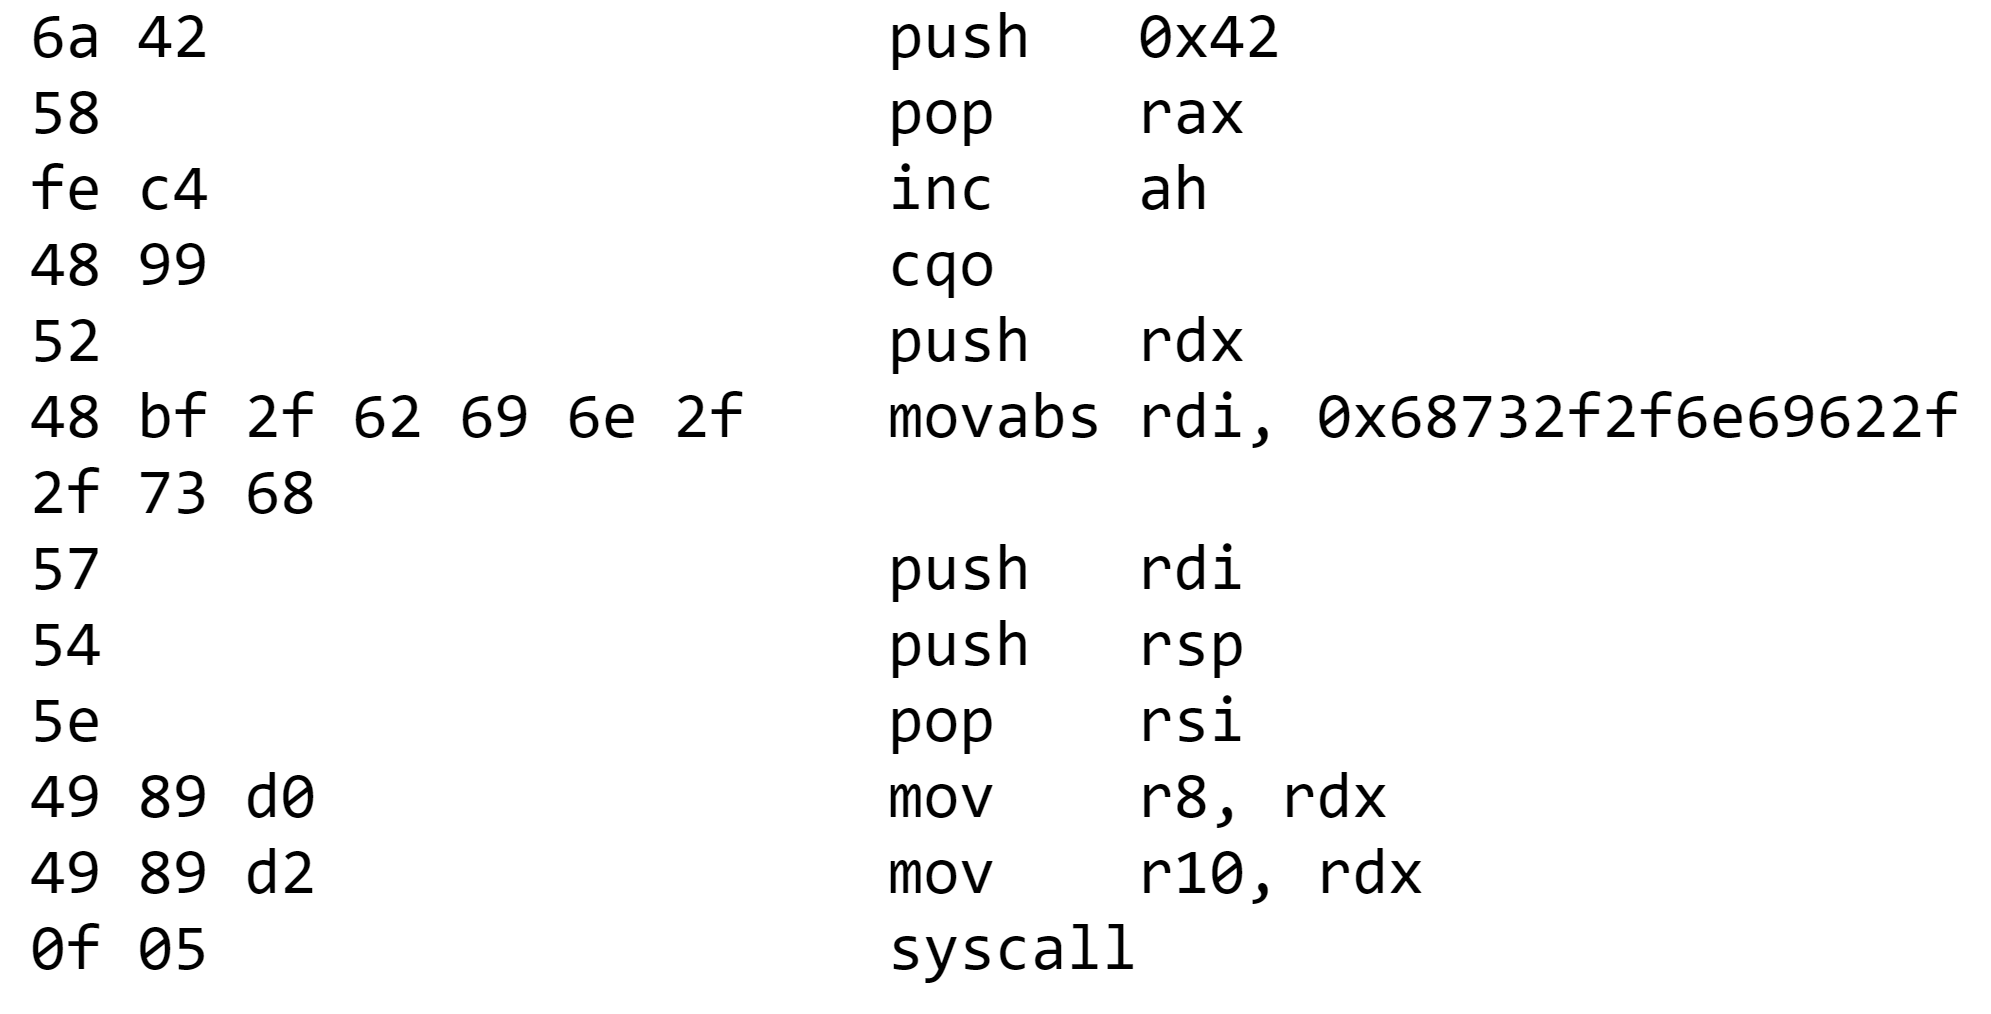
\includegraphics[width=0.9\textwidth,height=0.75\textheight,keepaspectratio]{images/shellstorm.png}
    \caption{Shellcode}
\end{figure}
\cite{shellstorm}

Die verwendeten Register und ihr Inhalt zum Zeitpunkt des Syscalls:

\begin{itemize}
    \item \textbf{RAX}: 322 (Nummer des Syscalls)
    \item \textbf{RDI}: 0x68732f2f6e69622f (Pfad der auszuführenden Datei: "/bin//sh")
    \item \textbf{RSI}: Pointer auf RDI (Zeiger auf den Pfad)
    \item \textbf{RDX}: 0 (Optional, nicht verwendet)
    \item \textbf{R10}: 0 (Optional, nicht verwendet)
    \item \textbf{R8}:  0 (Optional, nicht verwendet)
\end{itemize}
